\documentclass[12pt,a4paper]{report}
\usepackage{report}

\begin{document}
  % Cover and signature pages have no printed page numbers.
  \pagestyle{empty}
  \hypersetup{pageanchor=false}
  % Editable lines positioned to match Project Report.pdf, page 1.
\begin{frontpage}
  \CoverArtwork
  \FrontLine{cover-university}{\textbf{VISVESVARAYA TECHNOLOGICAL UNIVERSITY}}
  \FrontLine{cover-address}{\textbf{“JNANA SANGAMA” Belagavi – 590018, Karnataka}}
  \FrontLine{cover-degree-article}{\textbf{A}}
  \FrontLine{cover-phase-title}{\textbf{MAJOR PROJECT PHASE-I REPORT}}
  \FrontLine{cover-on}{\textbf{ON}}
  \FrontLine{cover-project-title}{\textbf{“}\textcolor[HTML]{00AE50}{\textbf{VEERDRISHTI:
    COMBAT VISION SYSTEM”}}}
  \FrontLine{cover-submission}{Submitted in partial fulfillment for the award of the
    degree in}
  \FrontLine{cover-degree}{\textcolor[HTML]{FF0000}{BACHELOR OF ENGINEERING}}
  \FrontLine{cover-in}{\textcolor[HTML]{FF0000}{IN}}
  \FrontLine{cover-branch}{\textcolor[HTML]{FF0000}{COMPUTER SCIENCE AND
    ENGINEERING}}
  \FrontLine{cover-submitted-by}{\textbf{Submitted by}}
  \FrontLine{cover-student-one}{\textcolor[HTML]{4471C4}{GAURAV CHAUHAN}}
  \FrontLine{cover-usn-one}{\textcolor[HTML]{4471C4}{1BH23CS024}}
  \FrontLine{cover-student-two}{\textcolor[HTML]{4471C4}{GAURAV SINGH}}
  \FrontLine{cover-usn-two}{\textcolor[HTML]{4471C4}{1BH23CS025}}
  \FrontLine{cover-guidance}{\textbf{Under the Guidance of}}
  \FrontLine{cover-guide-name}{\textbf{Ms. Sapna N}}
  \FrontLine{cover-guide-role}{Asst. Prof., Dept. of CSE}
  \FrontLine{cover-department}{\textbf{Department of Computer Science and Engineering}}
  \FrontLine{cover-institute}{\textbf{BANGALORE TECHNOLOGICAL INSTITUTE}}
  \FrontLine{cover-accreditation}{\textbf{(NAAC Accredited, An ISO 9001:2005 Certified
    Institute)}}
  \FrontLine{cover-address-line}{\textbf{Kodathi Village, Varthoor Hobli, Bengaluru East
    Taluk, Bengaluru Urban District}}
  \FrontLine{cover-city}{\textbf{Bengaluru, Karnataka – 560035.}}
  \FrontLine{cover-year}{\textbf{2025 – 2026}}
\end{frontpage}

  \begin{frontpage}
  \CertificateArtwork
  \FrontRule{certificate-department-rule}
  \FrontLine{certificate-department}{\textbf{DEPARTMENT OF COMPUTER SCIENCE AND ENGINEERING}}
  \FrontLine{certificate-heading}{\textcolor[HTML]{00AF50}{\textbf{CERTIFICATE}}}

  \FrontParagraph{certificate-body}{
    This is to certify that the Major Project Phase-I report entitled \textbf{“VEERDRISHTI: COMBAT
    VISION SYSTEM”} has been carried out by \textbf{GAURAV CHAUHAN [1BH23CS024]} and \textbf{GAURAV
    SINGH [1BH23CS025]}, bona fide students of \textbf{BANGALORE TECHNOLOGICAL INSTITUTE},
    Bengaluru, in partial fulfilment of the requirements for the award of \textbf{BACHELOR OF
    ENGINEERING} in \textbf{COMPUTER SCIENCE AND ENGINEERING} of \textbf{VISVESVARAYA TECHNOLOGICAL
    UNIVERSITY}, Belagavi, during the academic year \textbf{2025--2026}. It is certified that all
    corrections and suggestions indicated for Internal Assessment have been incorporated in the
    report. The Major Project Phase-I report has been approved as satisfying the academic
    requirements prescribed for the said degree.
  }

  % Signature lines and officials: retain the supplied college arrangement.
  \FrontRule{certificate-guide-rule}
  \FrontRule{certificate-coordinator-rule}
  \FrontLine{certificate-guide-name}{\textbf{Ms. Sapna N}}
  \FrontLine{certificate-coordinator-name}{\textbf{Mrs. M. Kalpana}}
  \FrontLine{certificate-guide-role}{Asst. Prof., Project Guide}
  \FrontLine{certificate-coordinator-role}{Asst. Prof., Project Coordinator}
  \FrontLine{certificate-guide-department}{Dept. of CSE}
  \FrontLine{certificate-coordinator-department}{Dept. of CSE}

  \FrontRule{certificate-hod-rule}
  \FrontRule{certificate-principal-rule}
  \FrontLine{certificate-hod-name}{\textbf{Dr. D. Jerline Sheebha Anni}}
  \FrontLine{certificate-principal-name}{\textbf{Dr. H. S. Nanda}}
  \FrontLine{certificate-hod-role}{Professor \& Head}
  \FrontLine{certificate-principal-role}{Principal}
  \FrontLine{certificate-hod-department}{Dept. of CSE}
\end{frontpage}

  \begin{frontpage}
  \DeclarationArtwork
  \FrontRule{declaration-department-rule}
  \FrontLine{declaration-department}{\textbf{DEPARTMENT OF COMPUTER SCIENCE AND ENGINEERING}}
  \FrontLine{declaration-heading}{\textcolor[HTML]{00AF50}{\textbf{DECLARATION}}}

  \FrontParagraph{declaration-body}{
    We, the students of pre-final year Computer Science and Engineering, Bangalore Technological
    Institute, Bengaluru, declare that the Major Project entitled \textbf{“VEERDRISHTI: COMBAT
    VISION SYSTEM”} is original work independently carried out by us under the guidance of
    \textbf{Ms. Sapna N}, Assistant Professor, \textbf{DEPARTMENT OF COMPUTER SCIENCE AND
    ENGINEERING, BANGALORE TECHNOLOGICAL INSTITUTE}, Bengaluru. This report is submitted in partial
    fulfilment of the requirements for the award of \textbf{BACHELOR OF ENGINEERING} in
    \textbf{COMPUTER SCIENCE AND ENGINEERING} of \textbf{VISVESVARAYA TECHNOLOGICAL UNIVERSITY},
    Belagavi, during the academic year \textbf{2025--2026}.

    We declare that this work has not formed the basis for the award of any other degree in this or
    any other institution or university. In keeping with ethical practice in reporting scientific
    information, due acknowledgements have been made wherever the findings of others have been
    cited.
  }

  \FrontRule{declaration-date-rule}
  \FrontLine{declaration-date}{Date:}
  \FrontLine{declaration-place}{Place: Bengaluru}

  \FrontLine{declaration-student-heading}{\textbf{Student Name}}
  \FrontLine{declaration-usn-heading}{\textbf{USN}}
  \FrontLine{declaration-signature-heading}{\textbf{Signature}}
  \FrontLine{declaration-student-one}{\textbf{GAURAV CHAUHAN}}
  \FrontLine{declaration-usn-one}{\textbf{1BH23CS024}}
  \FrontLine{declaration-signature-one}{\dotfill}
  \FrontLine{declaration-student-two}{\textbf{GAURAV SINGH}}
  \FrontLine{declaration-usn-two}{\textbf{1BH23CS025}}
  \FrontLine{declaration-signature-two}{\dotfill}
\end{frontpage}

  % Preliminary pages use Roman numbering.
  \pagenumbering{roman}
  \pagestyle{plain}
  \begin{frontpage}
  \label{front:acknowledgement}
  \FrontLine{acknowledgement-heading}{\textbf{ACKNOWLEDGEMENT}}

  \FrontParagraph{acknowledgement-body}{
    Any achievement, be it scholastic or otherwise, does not depend solely on individual efforts but
    on the guidance, encouragement and cooperation of intellectuals and elders. We would like to
    take this opportunity to thank them all.

    We express our gratitude to \textbf{Dr. H S Nanda}, Principal, for giving us this opportunity to
    enrich our knowledge.

    We express our immense gratitude to \textbf{Dr. D. Jerline Sheebha Anni}, Head of Department,
    CSE, for her unfailing encouragement and suggestions during our Major Project work.

    We thank \textbf{Mrs. M. Kalpana}, Assistant Professor and Major Project Coordinator, for her
    valuable advice, encouragement and suggestions.

    We thank \textbf{Ms. Sapna N}, Assistant Professor and Major Project Guide, for her valuable
    advice, encouragement and guidance throughout our Major Project work.

    We thank all the teaching and non-teaching staff of the Department of Computer Science and
    Engineering for their cooperation.

    Finally, we acknowledge our parents, guardians and friends for their support, feedback and
    indispensable help.
  }

  \FrontLine{acknowledgement-student-one}{\textbf{GAURAV CHAUHAN}}
  \FrontLine{acknowledgement-usn-one}{\textbf{1BH23CS024}}
  \FrontLine{acknowledgement-student-two}{\textbf{GAURAV SINGH}}
  \FrontLine{acknowledgement-usn-two}{\textbf{1BH23CS025}}
\end{frontpage}

  \begin{frontpage}
  \label{front:abstract}
  \FrontLine{abstract-heading}{\textbf{ABSTRACT}}

  % VTU guidelines: abstract must not exceed 100 words.
  \FrontParagraph{abstract-body}{
    VeerDrishti proposes an AI-enabled combat vision system that supports real-time situational
    awareness using wearable cameras and edge computing. Lightweight object detection identifies
    combatants, weapons, and vehicles, while augmented-reality overlays highlight potential threats.
    Visible and thermal image fusion is intended to improve perception in low-light and obscured
    environments. Synthetic data augmentation addresses limited training data, and open-vocabulary
    detection supports recognition of unfamiliar threats. The project focuses on reducing the burden
    of continuous manual surveillance and enabling timely, informed decisions. Phase-I establishes
    the literature review, requirements, system design, and development schedule; implementation and
    field evaluation remain future work.
  }
\end{frontpage}

  \begin{frontpage}
  \label{front:institute}
  \InstituteArtwork
  \FrontLine{institute-heading}{\textbf{VISION AND MISSION OF THE INSTITUTE}}
  \FrontLine{institute-name}{\textbf{BANGALORE TECHNOLOGICAL INSTITUTE}}
  \FrontLine{institute-vision-heading}{\textbf{VISION}}
  \FrontParagraph{institute-vision-body}{
    To evolve as a Centre of Excellence in Academics, Research and Development with an impact on
    Technological advancement to the Society.
  }

  \FrontLine{institute-mission-heading}{\textbf{MISSION}}
  \FrontParagraph{institute-mission-body}{
    M1 - To provide young prospective engineers with an environment for higher education and
    research.

    M2 - To mold students as responsible citizens with an attitude of using their knowledge for
    technological advancements.

    M3 - To uplift the downtrodden and improve the quality of life of fellow human beings.
  }
\end{frontpage}

  \begin{frontpage}
  \label{front:program}
  \ProgramArtwork
  \FrontLine{program-heading}{\textbf{VISION AND MISSION OF THE PROGRAM}}
  \FrontLine{program-name}{\textbf{COMPUTER SCIENCE AND ENGINEERING}}
  \FrontLine{program-vision-heading}{\textbf{VISION}}
  \FrontParagraph{program-vision-body}{
    To impart the best in academia \& research, empowering the students of Computer Science and
    Engineering by contributing their best for the society.
  }

  \FrontLine{program-mission-heading}{\textbf{MISSION}}
  \FrontParagraph{program-mission-body}{
    M1 - To impart updated theoretical and practical knowledge in computer science and engineering
    by creating an outstanding learning environment.

    M2 - To equip the students with wisdom in the discipline of computing and to apply their
    knowledge for benefiting the society.

    M3 - To enhance research collaborations for upliftment of computing professionals.
  }

  \FrontLine{program-peo-heading}{\textbf{PROGRAM EDUCATIONAL OBJECTIVES}}
  \FrontParagraph{program-peo-body}{
    PEO1 - To showcase strong technical proficiency in computer science fundamentals, empowering the
    design, development and implementation of innovative solutions that address real world
    challenges.

    PEO2 - To establish a solid foundation in the core concepts of computer science and engineering,
    while fostering a proactive attitude towards pursuing higher education and fulfilling industry
    demands.

    PEO3 - To embody professional ethics, strong communication skills, and leadership qualities that
    foster multidisciplinary excellence and career growth.

    PEO4 - To cultivate technical knowledge and research ability that inspire innovation, enabling
    the establishment of startups and fostering entrepreneurial success.

    PEO5 - To tackle societal, environmental and global challenges through the design of sustainable
    and efficient computer science and engineering-based systems that improve overall quality of
    life.
  }
\end{frontpage}

  % Split at paragraph boundaries rather than shrinking text below VTU spacing.
\begin{frontpage}
  \label{front:outcomes}
  \OutcomesArtwork
  \FrontLine{outcomes-heading}{\textbf{PROGRAM OUTCOMES}}

  \FrontParagraph{outcomes-body}{
    \textbf{1 Engineering knowledge:} Apply the knowledge of mathematics, science, engineering
    fundamentals, and an engineering specialization to the solution of complex engineering problems.

    \textbf{2 Problem analysis:} Identify, formulate, review research literature, and analyze
    complex engineering problems reaching substantiated conclusions using first principles of
    mathematics, natural sciences, and engineering sciences.

    \textbf{3 Design/development of solutions:} Design solutions for complex engineering problems
    and design system components or processes that meet the specified needs with appropriate
    consideration for public health and safety, and cultural, societal, and environmental
    considerations.

    \textbf{4 Conducting investigations of complex problems:} Use research-based knowledge and
    research methods including design of experiments, analysis and interpretation of data, and
    synthesis of the information to provide valid conclusions.

    \textbf{5 Modern tool usage:} Create, select, and apply appropriate techniques, resources, and
    modern engineering and IT tools including prediction and modelling to complex engineering
    activities with an understanding of the limitations.

    \textbf{6 The Engineer and society:} Apply reasoning informed by contextual knowledge to assess
    societal, health, safety, legal and cultural issues and the consequent responsibilities relevant
    to professional engineering practice.

    \textbf{7 Environment and sustainability:} Understand the impact of professional engineering
    solutions in societal and environmental contexts, and demonstrate the knowledge of, and need for
    sustainable development.
  }
\end{frontpage}

\begin{frontpage}
  \label{front:outcomes-end}
  \OutcomesArtwork
  \FrontLine{outcomes-heading}{\textbf{PROGRAM OUTCOMES}}

  \FrontParagraph{outcomes-body}{
    \textbf{8 Ethics:} Apply ethical principles and commit to professional ethics and
    responsibilities and norms of engineering practice.

    \textbf{9 Individual and team work:} Function effectively as an individual, and as a member or
    leader in diverse teams, and in multi-disciplinary settings.

    \textbf{10 Communication:} Communicate effectively on complex engineering activities with the
    engineering community and with society at large, such as being able to comprehend and write
    effective reports and design documentation, make effective presentations, and give and receive
    clear instructions.

    \textbf{11 Project management and finance:} Demonstrate knowledge and understanding of
    engineering and management principles and apply these to one's own work, as a member and leader
    in a team, to manage projects and in multi-disciplinary environments.

    \textbf{12 Life-long learning:} Recognize the need for and have the preparation and ability to
    engage in independent and life-long learning in the broadest context of technological change.
  }
\end{frontpage}

  \begin{frontpage}
  \label{front:specific_outcomes}
  \SpecificOutcomesArtwork
  \FrontLine{specific-outcomes-heading}{\textbf{PROGRAM SPECIFIC OUTCOMES}}

  \FrontParagraph{specific-outcomes-body}{
    PSO1 - Demonstrate proficiency in computer education by applying principles of mathematics,
    science \& engineering along with technical expertise.

    PSO2 - Equip proficiency in computer science and engineering employing the principles of
    communication networks, database management systems, computing systems \& standard software
    development practices to cater to technical growth.

    PSO3 - Develop proficiency in analytical skills, research \& innovation contributing effectively
    as per industry requirements by delivering effective socio-economic skills for the advancement
    of technology.
  }
\end{frontpage}

  \begin{frontpage}
  \label{front:contents}
  \FrontLine{contents-index-heading}{\textbf{INDEX}}
  \FrontLine{contents-acknowledgement}{\textbf{ACKNOWLEDGEMENT}}
  \FrontLine{contents-abstract}{\textbf{ABSTRACT}}
  \FrontLine{contents-institute}{\textbf{VISION AND MISSION OF THE INSTITUTE}}
  \FrontLine{contents-program}{\textbf{VISION AND MISSION \& PEO OF THE PROGRAM}}
  \FrontLine{contents-outcomes}{\textbf{PROGRAM OUTCOMES}}
  \FrontLine{contents-specific-outcomes}{\textbf{PROGRAM SPECIFIC OUTCOMES}}
  \FrontLine{contents-table-of-contents}{\textbf{TABLE OF CONTENTS}}
  \FrontLine{contents-figures}{\textbf{LIST OF FIGURES}}
  \FrontLine{contents-tables}{\textbf{LIST OF TABLES}}
  \FrontLine{contents-acknowledgement-page}{\hfill\textbf{\pageref{front:acknowledgement}}\hfill}
  \FrontLine{contents-abstract-page}{\hfill\textbf{\pageref{front:abstract}}\hfill}
  \FrontLine{contents-institute-page}{\hfill\textbf{\pageref{front:institute}}\hfill}
  \FrontLine{contents-program-page}{\hfill\textbf{\pageref{front:program}}\hfill}
  \FrontLine{contents-outcomes-page}{\hfill\textbf{\PageRange{front:outcomes}{front:outcomes-end}}\hfill}
  \FrontLine{contents-specific-outcomes-page}{\hfill\textbf{\pageref{front:specific_outcomes}}\hfill}
  \FrontLine{contents-table-of-contents-page}{\hfill\textbf{\PageRange{front:contents}{front:contents-end}}\hfill}
  \FrontLine{contents-figures-page}{\hfill\textbf{\pageref{front:figures}}\hfill}
  \FrontLine{contents-tables-page}{\hfill\textbf{\pageref{front:tables}}\hfill}
  \FrontRule{contents-divider}
  \FrontLine{contents-body-heading}{\textbf{TABLE OF CONTENTS}}
  \FrontLine{contents-chapter-label}{\textbf{Chapter}}
  \FrontLine{contents-number-label}{\textbf{No.}}
  \FrontLine{contents-chapters-label}{\textbf{CHAPTERS}}
  \FrontLine{contents-page-label}{\textbf{Page No.}}
  \ContentsChapter{introduction}{ch:introduction}{end:introduction}
  \ContentsRow{overview}{sec:overview}{end:overview}
  \ContentsRow{problem}{sec:problem}{end:problem}
  \ContentsRow{motivation}{sec:motivation}{end:motivation}
  \ContentsRow{objectives}{sec:objectives}{end:objectives}
  \ContentsRow{methodology}{sec:methodology}{end:methodology}
  \ContentsRow{sdg}{sec:sdg}{end:sdg}
  \ContentsRow{feasibility}{sec:feasibility}{end:feasibility}
  \ContentsRow{work}{sec:work}{end:work}
  \ContentsChapter{literature}{ch:literature}{end:literature}
  \ContentsRow{base}{sec:base}{end:base}
  \ContentsRow{supplementary}{sec:supplementary}{end:supplementary}
\end{frontpage}

\begin{frontpage}
  \label{front:contents-end}
  \FrontPageTwoContents
  \ContentsRow{comparison}{sec:comparison}{end:comparison}
  \ContentsChapter{requirements}{ch:requirements}{end:requirements}
  \ContentsRow{functional}{sec:functional}{end:functional}
  \ContentsRow{nonfunctional}{sec:nonfunctional}{end:nonfunctional}
  \ContentsRow{hardware}{sec:hardware}{end:hardware}
  \ContentsRow{software}{sec:software}{end:software}
  \ContentsChapter{design}{ch:design}{end:design}
  \ContentsRow{architecture}{sec:architecture}{end:architecture}
  \ContentsRow{workflow}{sec:workflow}{end:workflow}
  \ContentsChapter{scheduling}{ch:scheduling}{end:scheduling}
  \ContentsRow{gantt}{sec:gantt}{end:gantt}
  \ContentsRow{progress}{sec:progress}{end:progress}
  \ContentsChapter{conclusion}{ch:conclusion}{end:conclusion}
  \FrontLine{contents-references}{\textbf{REFERENCES}}
  \FrontLine{contents-references-page}{\hfill\textbf{\PageRange{ch:references}{end:references}}\hfill}
\end{frontpage}

  \begin{frontpage}
  \label{front:figures}
  \FrontLine{figures-heading}{\textbf{LIST OF FIGURES}}
  \FrontLine{figures-number-label}{\textbf{Fig. No.}}
  \FrontLine{figures-title-label}{\textbf{Title of the Figure}}
  \FrontLine{figures-page-label}{\textbf{Page No.}}
  \FrontLine{figures-architecture-number}{\ref{fig:architecture}}
  \FrontLine{figures-architecture-title}{\nameref{fig:architecture}}
  \FrontLine{figures-architecture-page}{\pageref{fig:architecture}}
  \FrontLine{figures-workflow-number}{\ref{fig:workflow}}
  \FrontLine{figures-workflow-title}{\nameref{fig:workflow}}
  \FrontLine{figures-workflow-page}{\pageref{fig:workflow}}
  \FrontLine{figures-gantt-number}{\ref{fig:gantt}}
  \FrontLine{figures-gantt-title}{\nameref{fig:gantt}}
  \FrontLine{figures-gantt-page}{\pageref{fig:gantt}}
\end{frontpage}

  \begin{frontpage}
  \label{front:tables}
  \FrontLine{tables-heading}{\textbf{LIST OF TABLES}}
  \FrontLine{tables-number-label}{\textbf{Table No.}}
  \FrontLine{tables-title-label}{\textbf{Title of the Table}}
  \FrontLine{tables-page-label}{\textbf{Page No.}}
  \FrontLine{tables-work-number}{\ref{tab:work}}
  \FrontLine{tables-work-title}{\nameref{tab:work}}
  \FrontLine{tables-work-page}{\pageref{tab:work}}
  \FrontLine{tables-comparison-number}{\ref{tab:comparison}}
  \FrontLine{tables-comparison-title}{\nameref{tab:comparison}}
  \FrontLine{tables-comparison-page}{\PageRange{tab:comparison}{end:comparison}}
\end{frontpage}


  % Body chapters and references use Arabic numbering.
  \pagenumbering{arabic}
  \hypersetup{pageanchor=true}
  \pagestyle{report}
  \chapter{INTRODUCTION}\label{ch:introduction}

\section{Overview}\label{sec:overview}
Modern warfare has transitioned into an increasingly data-driven environment where split-second
decisions are critical for survival and mission success. The sheer volume of visual information from
surveillance feeds, drones, and tactical environments often overwhelms personnel, leading to
cognitive fatigue and a higher margin for error. Manual threat assessment is no longer sufficient to
ensure the safety and tactical superiority of ground units in high-stress scenarios. Consequently,
there is an urgent need for intelligent, autonomous systems that can process vast amounts of
real-time visual data to provide actionable insights and enhance situational awareness. \vspace{6pt}

VeerDrishti is an AI-enabled combat vision system designed to bridge this gap by providing soldiers
with a persistent, intelligent observer through a camera-integrated solution. By leveraging
state-of-the-art computer vision models and edge computing, the system autonomously identifies enemy
combatants, vehicles, and weapons. The primary objective is to offload the mental burden of constant
monitoring from the soldier, allowing them to focus on strategic execution. Developed as a
lightweight solution suitable for deployment on wearable hardware, the system aims to transform how
visual data is utilized on the front lines of national security. \vspace{6pt}

The project incorporates sophisticated methodologies to ensure reliability under diverse and
challenging battlefield conditions. It utilizes multimodal image fusion—combining visible and
thermal spectrums—to maintain high detection accuracy in low-light or obscured environments.
Furthermore, by implementing edge-optimized architectures and advanced feature fusion techniques,
the system achieves high-speed inference without compromising precision. This integration of
versatile object detection and robust information processing ensures that the system remains a
reliable asset, offering a significant technological advantage in modern combat and defense
operations.

\label{end:overview}
\section{Problem Statement}\label{sec:problem}
The problem statement is to address the challenges of managing vast real-time visual data in modern
battlefield environments, where manual monitoring is slow, error-prone, and inefficient; in order to
enhance situational awareness and tactical decision-making, an AI-powered combat vision system is
proposed to automatically detect, classify, and assess threats in real time, improving response
speed and operational efficiency.

\label{end:problem}
\section{Motivation}\label{sec:motivation}
The motivation for VeerDrishti is to minimize casualties and save lives by providing an intelligent,
persistent observer in combat environments. Modern warfare involves overwhelming visual data that
leads to cognitive fatigue, increasing the risk of fatal human error. The system serves as a
technological safeguard, enhancing personnel safety and protecting national security forces during
high-stress operations.

\subsection{Scope}
The scope of the project is to develop an autonomous, real-time vision system designed to detect
enemy personnel, weapons, and vehicles in tactical environments. The technical implementation will
focus on developing a lightweight system, optimized for localized inference on mobile edge devices.

\subsection{Purpose}
The purpose of the project is to provide an autonomous, intelligent observer that delivers real-time
situational awareness in high-stress combat environments. By automating threat detection and
mitigating cognitive fatigue, the system serves as a technological safeguard dedicated to achieving
the project's core mission: minimizing casualties and saving lives.

\subsection{Applicability}
The project will be applicable in active combat operations, border surveillance, and high-risk
tactical missions where ground units require instantaneous threat identification. The edge-optimized
architecture will ensure reliability in signal-denied zones and low-visibility environments, serving
as a critical force multiplier for national security personnel. \vspace{6pt}

Beyond defense, the system's ability to automate hazard detection will be directly transferable to
emergency response and disaster management, fulfilling the mandate to minimize casualties and save
lives.

\label{end:motivation}
\section{Objectives}\label{sec:objectives}
The project's primary objectives are to develop a lightweight, real-time combat vision system that
can be deployed on wearable hardware, capable of autonomously detecting and classifying threats in
dynamic battlefield environments. \vspace{6pt}

Specific objectives for the project include:
\begin{enumerate}[label=\roman*.]
  \item Implement a lightweight real-time object detection model.
  \item Enable on-screen visual highlighting of identified threats.
  \item Optimize system performance for low latency and smooth operation.
  \item Evaluate accuracy and response time under simulated field conditions.
  \label{end:objectives}
\end{enumerate}
\section{Methodology}\label{sec:methodology}
The project adopts a hybrid deep-learning approach that integrates generative data augmentation with
edge-optimized multimodal fusion. Initially, the system utilizes a Generative Adversarial Network
(GAN) to synthesize high-quality military training data, addressing scarcity in combat-specific
datasets. For real-time execution, the project implements a lightweight detection architecture, such
as EfficientDet or YOLOv10, optimized for low-latency performance on edge devices like smartphones
or Raspberry Pi. To ensure reliability in varying field conditions, the methodology incorporates
multimodal image fusion, specifically merging RGB texture with Infrared (thermal) edge data using a
fine-grained region attention mechanism. This ensures robust target classification even during night
operations or in cluttered environments. Furthermore, the system leverages a vision-language model
(like Florence v2) for zero-shot detection, allowing the identification of "unseen" or novel threats
through natural language supervision. Post-detection, the pipeline filters data and applies an
Augmented Reality (AR) overlay to highlight threats instantly, while securing all mission metadata
in a local storage layer for subsequent auditing.

\label{end:methodology}
\section{Sustainable Development Goal Relevance}\label{sec:sdg}
The project aligns with United Nations Sustainable Development Goal 16: Peace, Justice, and Strong
Institutions.

\textbf{Target 16.1: Significantly reduce all forms of violence and related death rates everywhere}

VeerDrishti will enhance battlefield situational awareness by detecting and tracking potential
threats in real time. This capability will enable defense personnel to respond faster and make more
informed decisions during combat situations. By improving awareness and reaction time, the system
will help reduce operational risks and potentially decrease casualties. \\

\textbf{Target 16.3: Promote the rule of law at the national and international levels and ensure
  equal access to justice for all}

VeerDrishti will record visual data during operations, enabling improved mission analysis and
operational review. It will support evidence-based evaluation of decisions made during missions.
Such recorded data could also assist investigations related to violations of international
humanitarian law, including potential war crimes. \\

\textbf{Target 16.A: Strengthen relevant national institutions, including through international
  cooperation, for building capacity at all levels, in particular in developing countries, to
  prevent violence and combat terrorism and crime}

VeerDrishti will integrate AI-based detection and tracking technologies, strengthening the
technological capacity of national security institutions. The project will support peacekeeping
operations and the protection of national interests.

\label{end:sdg}
\section{Feasibility Study}\label{sec:feasibility}
The feasibility of the proposed combat vision system is assessed across technical, operational, and
economic dimensions.

\subsection{Technical Feasibility}
The proposed system is technically feasible using existing smartphone hardware and computer vision
frameworks. Modern phones provide high-resolution cameras, sufficient processing power, and GPU
support for real-time object detection. Lightweight AI models can be optimized for edge deployment,
enabling on-device threat detection without requiring complex external hardware.

\subsection{Operational Feasibility}
The system can be integrated into existing helmet setups with minimal modification, using a mounted
smartphone as both camera and display interface. It reduces cognitive load by automating threat
detection and visual highlighting. Basic training would enable personnel to interpret AR overlays
effectively in dynamic environments.

\subsection{Economic Feasibility}
Using commercially available smartphones significantly lowers development and deployment costs
compared to specialized military hardware. Open-source AI frameworks further reduce software
expenses. The prototype approach minimizes initial investment, making the system cost-effective for
research, testing, and potential scalable improvements in future versions.

\label{end:feasibility}
\section{Work Distribution}\label{sec:work}
\begin{table}[h]
  \centering
  \caption{Work Distribution Among Team Members}\label{tab:work}
  \begin{tabular}{lll}
    \toprule
    \textbf{Name} & \textbf{Tasks} \\
    \midrule
    Gaurav Chauhan & Literature Survey and Report Writing \\
    Gaurav Singh & Literature Survey and Slide Preparation \\
    \bottomrule
  \end{tabular}
\end{table}
\label{end:work}\label{end:introduction}

  \chapter{LITERATURE REVIEW}\label{ch:literature}

\section{Base Paper}\label{sec:base}
\subsection{Military target detection method based on EfficientDet and Generative Adversarial
  Network}
\textbf{Authors:} X. Zhuang, D. Li, Y. Wang, and K. Li \\
\textbf{Journal:} Engineering Applications of Artificial Intelligence \\
\textbf{Published:} June 2024 \\
\textbf{DOI:} 10.1016/j.engappai.2024.107896 \\

\textbf{Summary:} This paper proposes a novel method for military target detection by integrating
EfficientDet, a state-of-the-art object detection model, with a Generative Adversarial Network (GAN)
to enhance the training data. The authors demonstrate that this approach significantly improves
detection accuracy, especially in scenarios with limited training data. The method is evaluated on a
military target dataset, showing superior performance compared to traditional detection methods. \\

\textbf{Methodology:} The authors first use EfficientDet to detect targets in the original dataset.
Then, they employ a GAN to generate synthetic images of military targets, which are added to the
training set. The enhanced dataset is used to retrain the EfficientDet model, resulting in improved
detection performance. \\

\textbf{Results:} The method achieved 92.8\% mean Average Precision (mAP) on a custom military
dataset, outperforming YOLOv3 and YOLOv5. It maintained real-time performance (15 FPS) on the test
hardware. In complex scenarios (dim lighting, occlusions), the model still achieved over 90\%
detection accuracy.

\label{end:base}
\section{Supplementary Papers}\label{sec:supplementary}

\subsection{Real-Time Versatile Object Detection With High Accuracy And Reduced Information Loss
  During Wartime}
\textbf{Authors:} D N, Shylaja and Dhanalakshmi, M. \\
\textbf{Conference:} 2024 International Conference on Integration of Emerging Technologies for the
Digital World (ICIETDW) \\
\textbf{Published:} September 2024 \\
\textbf{DOI:} 10.1109/ICIETDW61607.2024.10939768 \\

\begingroup\emergencystretch=2em
  \textbf{Summary:} A state-of-the-art object detection system for analyzing camera or drone
  footage. Designed to identify battlefield threats such as vehicles, weapons, and combatants. Uses
  a vision-language model, combining images and natural language descriptions for better
  understanding and classification. \\
\par\endgroup

\textbf{Methodology:} CLIP links images with text descriptions, enabling detection of new objects
without large labeled datasets. SPPELAN Pooling module that ensures fixed feature representation
with minimal information loss. N-gram \& GLIP Labeler extracts noun phrases and creates
pseudo-boundaries for objects to generate training data. K-means Clustering groups similar image
regions to improve efficiency in cluttered scenes. \\

\textbf{Results:} Compared with Grounding DINO on the Microsoft COCO dataset, the system showed
better efficiency. Lower complexity (48M parameters vs 172M), higher accuracy (AP 35 vs 25.6) and
faster framerate (17.6 FPS vs 1.5 FPS), making it suitable for realtime deployment.

\subsection{EDNet: Edge-Optimized Small Target Detection in UAV Imagery - Faster Context Attention,
  Better Feature Fusion, and Hardware Acceleration}
\textbf{Authors:} Song, Zhifan and Zhang, Yuan and Ebayyeh, Abd Al Rahman M. Abu \\
\textbf{Conference:} 2024 IEEE Smart World Congress (SWC) \\
\textbf{Published:} December 2024 \\
\textbf{DOI:} 10.1109/SWC62898.2024.00141 \\


\textbf{Summary:} EDNet is a deep-learning framework for detecting small objects in UAV/drone
imagery. Built on YOLOv10 and optimized for edge computing, allowing efficient use on mobile and
low-power devices. The model is scalable, with 7 sizes ranging from Tiny (lightweight) to XL (high
performance). \\

\textbf{Methodology:} C2f-FCA Block uses faster context attention to extract features with lower
computational complexity. WIoUv3 Loss Function helps the model focus on high-quality samples and
ignore noisy data. Optimized Deployment uses CoreML, TensorRT, and OpenVINO for high-speed
performance across different processors. \\

\textbf{Results:} EDNet outperformed models like YOLOv8 and YOLOv10 in accuracy and speed. Higher
Accuracy: Up to 5.6\% improvement in mAP$_{50}$ compared to YOLOv10 with fewer parameters. Better
Efficiency: EDNet-M surpassed YOLOv10-X while using 39.6\% fewer parameters. Real-Time Performance:
16–55 FPS on iPhone 12; EDNet-Tiny runs 3 times faster on Raspberry Pi 5.

\subsection{Multi-modal action recognition via advanced image fusion techniques for cyber-physical
  systems}
\textbf{Authors:} Shou, Zaiyong and Zhu, Daoyu \\
\textbf{Journal:} Frontiers in Physics \\
\textbf{Published:} August 2025 \\
\textbf{DOI:} 10.3389/fphy.2025.1576591 \\

\textbf{Summary:} A framework for cyber-physical systems such as autonomous vehicles and smart
surveillance. It introduces MSAF-Net, a system for human action recognition. It combines multiple
visual data types like RGB, depth, and thermal images for more accurate detection. \\

\textbf{Methodology:} Multi-Scale Attention Fusion extracts features at different detail levels and
prioritizes the most relevant ones. Cross-Level Feature Interaction allows network layers to share
information, preserving fine details and global structure. Adaptive Fusion Strategy ensures clear
and consistent fused data using semantic and structural guidance. \\

\begingroup\emergencystretch=2em
  \textbf{Results:} MSAF-Net outperformed existing state-of-the-art models across four major
  datasets. It achieved 91.54\% accuracy on UCF101 and 92.14\% on ActivityNet. The model remains
  robust even if one sensor fails and can be pruned for faster performance on low-power hardware.
\par\endgroup

\subsection{Static Early Fusion Techniques for Visible and Thermal Images to Enhance Convolutional
  Neural Network Detection: A Performance Analysis}
\textbf{Authors:} Heredia-Aguado, Enrique and Cabrera, Juan José and Jiménez, Luis Miguel and
Valiente, David and Gil, Arturo \\
\textbf{Journal:} Remote Sensing \\
\textbf{Published:} March 2025 \\
\textbf{DOI:} 10.3390/rs17061060 \\

\textbf{Summary:} The paper discusses fusion of RGB images and infrared data. It compares early and
middle fusion techniques to combine both sources to create a more robust real-time detection system
for mobile robots and UAVs in search-and-rescue or security missions. \\

\textbf{Methodology:} Early Fusion Methods like RGBT, HSVT, VTHS, and VT were tested to combine RGB
and thermal data. Alignment correction was implemented via optical-flow-based affine transformation
to fix RGB–thermal misalignment in the KAIST dataset. Images weere enhanched by applying CLAHE to
improve contrast and grayscale range in thermal and visible images. \\

\textbf{Results:} Best results came from using separate models for day and night. In night
conditions, VT and VTHS fusion performed best, relying on brightness and thermal data instead of
color. In daylight, RGBT fusion worked best by using color information effectively. Simple early
fusion methods often outperformed complex middle fusion models, which were more prone to
overfitting.

\subsection{Infrared-Visible Image Fusion Meets Object Detection: Towards Unified Optimization for
  Multimodal Perception}

\textbf{Authors:} Xiang, Xiantai and Zhou, Guangyao and Niu, Ben and Pan, Zongxu and Huang, Lijia
and Li, Wenshuai and Wen, Zixiao and Qi, Jiamin and Gao, Wanxin \\
\textbf{Journal:} Remote Sensing \\
\textbf{Published:} November 2025 \\
\textbf{DOI:} 10.3390/rs17213637 \\

\textbf{Summary:} UniFusOD is an end-to-end framework for infrared–visible image fusion and object
detection. It combines visible images (rich texture and color) with infrared images (strong edges in
low light). The system produces a single fused image optimized for clear visualization and accurate
detection. \\

\textbf{Methodology:} FRA Mechanism uses multiple convolution kernels to capture both fine details
and larger semantic features. UnityGrad Optimization balances fusion and detection gradients,
preventing conflicts so both tasks train effectively. \\

\textbf{Results:} UniFusOD outperformed several state-of-the-art models on multiple datasets. Better
Detection: Improved mAP by 0.8 (DroneVehicle) and 1.9 (M3FD). Superior Fusion: Produced images with
higher information content and better structure. Robust Performance: Particularly effective at
detecting small targets in complex environments.

\subsection{An Efficient and Lightweight Deep Learning Model for Human Activity Recognition Using
  Smartphones}

\textbf{Authors:} A. Ankita, S. Rani, H. Babbar, S. Coleman, A. Singh, and H. M. Aljahdali \\
\textbf{Journal:} Sensors \\
\textbf{Published:} June 2021 \\
\textbf{DOI:} 10.3390/s21113845 \\

\textbf{Summary:} Presents an efficient and lightweight deep learning model for recognizing human
activities using smartphone sensors. It addresses the limitations of traditional pattern recognition
by using automated feature extraction, which is essential for applications in healthcare, elderly
monitoring, and sports science. \\

\textbf{Methodology:} The proposed CNN-LSTM architecture combines convolutional layers for automated
feature extraction with LSTM units for processing temporal sequences. The model was trained using
the UCI-HAR dataset from Samsung Galaxy S2 smartphones, employing Gaussian standardization to
preprocess raw accelerometer and gyroscope signals. \\

\textbf{Results:} UThe CNN-LSTM model achieved a high recognition accuracy of 97.89\%. It proved to
be more robust and capable than traditional algorithms, demonstrating that combining spatial feature
learning with temporal sequence interpretation effectively identifies activities like walking,
sitting, and standing while remaining lightweight for mobile deployment.

\subsection{Detection and classification of different weapon types using deep learning}

\textbf{Authors:} V. Kaya, S. Tuncer, and A. Baran \\
\textbf{Journal:} Applied Sciences \\
\textbf{Published:} August 2021 \\
\textbf{DOI:} 10.3390/app11167535 \\

\textbf{Summary:} Proposes a deep learning model for the automatic detection and classification of
seven distinct handheld weapon types. It aims to support security forces by providing a proactive
control system that can identify threatening objects in real-time surveillance to prevent criminal
activities. \\

\textbf{Methodology:} Based on the VGGNet architecture, the proposed CNN model uses 25 layers and
337,671 parameters. A new dataset of 5,214 images (assault rifles, pistols, grenades, etc.) was
curated from the internet and preprocessed using gray formatting and background cleaning for
training via the Keras library. \\

\textbf{Results:} The model achieved 98.40\% classification accuracy, significantly outperforming
VGG-16 (89.75\%), ResNet50 (93.70\%), and ResNet-101 (83.33\%). It successfully identified weapons
with low loss rates (0.052), proving highly effective for real-world deployment on low-cost
computers due to its reduced layer complexity and fast training time.

\subsection{Review of models for estimating 3D human pose using deep learning}

\textbf{Authors:} S. Salisu, K. U. Danyaro, M. Nasser, I. M. Hayder, and H. A. Younis \\
\textbf{Journal:} PeerJ Computer Science \\
\textbf{Published:} February 2025 \\
\textbf{DOI:} 10.7717/peerj-cs.2574 \\

\textbf{Summary:} Evaluates the latest deep learning-based models for 3D human pose estimation
(HPE). It explores the evolution from 2D to 3D positioning of articulated joints, highlighting key
industrial applications in healthcare telerehabilitation, security surveillance, gaming, and action
recognition. \\

\textbf{Methodology:} Researchers followed the PRISMA protocol to systematically search Scopus, Web
of Science, and IEEE databases for articles published between 2014 and 2024. They assessed 30
leading studies based on neural network architectures, benchmark datasets (like Human 3.6M), and
metrics like Mean Per Joint Position Error. \\

\textbf{Results:} The review found that while deep learning has significantly advanced 3D HPE, major
challenges persist in handling occlusion and real-time processing. Findings emphasize the success of
multi-view and sensor-fusion techniques, providing a roadmap for future research toward more robust,
generalized models for complex environments.

\subsection{PDGV-DETR: Object detection for secure on-site weapon and personnel location based on
  dynamic convolution and cross-scale semantic fusion}

\textbf{Authors:} N.Li,P.Xin,J.Tian,X.Bai,H.Ding,Z.Xiao,andQ.Liu \\
\textbf{Journal:} Remote Sensing \\
\textbf{Published:} February 2026 \\
\textbf{DOI:} 10.3390/s26051542 \\

\textbf{Summary:} : Proposes PDGV-DETR, a framework for precise weapon and personnel detection in
static security surveillance images. It addresses challenges like object occlusion and complex
backgrounds, which often cause general detection models to fail in public safety scenarios such as
school or subway monitoring. \\

\textbf{Methodology:} Themodel optimizes detection through three units: a dynamic hierarchical
channel interaction convolution module for occluded objects, an improved bidirectional hybrid
feature pyramid network for cross-scale fusion, and a global semantic weaving network to better
distinguish objects from complex backgrounds in static images. \\

\textbf{Results:} PDGV-DETR achieved a peak mAP$_{50}$ of 85.9\% on conflict scene datasets and
93.0\% on weapon-specific datasets. It demonstrated a statistically significant improvement over
RT-DETR and DeformableDETR, balancing high positioning accuracy with computational efficiency for
real-time video surveillance applications.

\subsection{Edge-optimized threat detection with Florence v2 for autonomous surveillance in
  resource-constrained environments}

\textbf{Authors:} C. Konar, D. Das, D. S., K. Jc, and S. Singh \\
\textbf{Journal:} PeerJ Computer Science \\
\textbf{Published:} March 2026 \\
\textbf{DOI:} 10.7717/peerj-cs.3579 \\

\textbf{Summary:} Introduces a portable, edge-optimized surveillance system designed to detect
modern security threats like hidden weapons and drones. By leveraging the Florence v2
Vision-Language Transformer, it aims to provide militarygrade object detection in
resource-constrained environments like remote borders or civilian infrastructure. \\

\textbf{Methodology:} Researchers adapted the Florence v2 model using Parameter Efficient
Fine-Tuning (PEFT) and LowRank Adaptation (LoRA). The system was trained on 12,000 images, including
GAN-generated synthetic data, and deployed on a Raspberry Pi 5 with an ESP32-S2 module for wireless
alerts via the ESP-NOW protocol. \\

\textbf{Results:} The final model achieved 88.01\% accuracy, outperforming YOLOv8 and FRCNN. It
attained a mAP$_{50}$ score of 64.83 while maintaining high efficiency on edge hardware, utilizing
only 38.4\% of the Raspberry Pi's RAM and 50.9\% of its CPU power per 16.6ms frame.


\label{end:supplementary}
\pagebreak
\section{Comparison Table}\label{sec:comparison}
\begingroup
  \renewcommand{\arraystretch}{1.5}
  \setlength{\tabcolsep}{5.9pt}
  \begin{longtable}{p{1.21cm} p{3cm} p{3cm} p{3cm} p{3cm}}
    \caption{Comparison Table of Research Papers}\label{tab:comparison} \\

    \toprule
    \textbf{Sl. No.} &
    \textbf{Paper Title} &
    \textbf{Objective} &
    \textbf{Methodology} &
    \textbf{Core Idea} \\
    \midrule
    \endfirsthead

    \toprule
    \textbf{Sl. No.} &
    \textbf{Paper Title} &
    \textbf{Objective} &
    \textbf{Methodology} &
    \textbf{Core Idea} \\
    \midrule
    \endhead

    \midrule
    \multicolumn{5}{r}{\textit{Continued on next page}} \\
    \midrule
    \endfoot

    \bottomrule
    \endlastfoot

    \cite{base_paper} &
    Military target detection method based on EfficientDet and Generative Adversarial Network &
    To detect targets in low visibility, noisy, or data-scarce combat zones &
    EfficientDet-D0 + Dual-Discriminator GAN &
    Uses GANs to generate synthetic military training data and BiFPN for feature fusion \\

    \cite{supplementary_paper_1} &
    Real-Time Versatile Object Detection With High Accuracy and Reduced Information Loss During Wartime &
    To detect unseen or new battlefield threats without manual re-labeling &
    CLIP Encoder + Modified C2f-Darknet &
    Uses pseudo-boundary labeling for zero-shot detection and combines vision and language \\

    \cite{supplementary_paper_2} &
    EDNet: Edge-Optimized Small Target Detection in UAV Imagery — Faster Context Attention, Better Feature Fusion, and Hardware Acceleration &
    To enable high-speed detection of tiny objects on low-power drone hardware &
    YOLOv10 + Faster Context Attention (C2fFCA) &
    Uses XSmall detection layer for small object detection with hardware acceleration optimizations \\

    \cite{supplementary_paper_3} &
    Multi-modal action recognition via advanced image fusion techniques for cyber-physical systems &
    To recognize human/combatant actions accurately even if one sensor fails &
    MSAF-Net (Multi-Scale Attention-Guided Fusion) &
    Dynamically prioritizes sensor data and switches to backup sensors when needed \\

    \cite{supplementary_paper_4} &
    Static early fusion techniques for visible and thermal images to enhance convolutional neural network detection: A performance analysis &
    To find the most efficient way to merge RGB and infrared data for robots &
    YOLOv8 + Early Fusion &
    Compresses 4-channel data into 3-channel for efficiency processing and uses CLAHE for contrast enhancement \\

    \cite{supplementary_paper_5} &
    Infrared-visible image fusion meets object detection: Towards unified optimization for multimodal perception &
    To solve gradient conflicts when training fusion and detection together &
    UniFusOD &
    Use Fine-Grained Region Attention (FRA) mechanism and unified framework to fuse RGB and infrared images for accurate detection \\

    \cite{supplementary_paper_6} &
    An Efficient and Lightweight Deep Learning Model for Human Activity Recognition Using Smartphones &
    To develop an efficient and lightweight model for identifying human activities using smartphone-based sensor data &
    CNN + Long Short-Term Memory (LSTM) &
    Integrating spatial and temporal deep learning architectures to automate feature extraction from raw sensor data \\

    \cite{supplementary_paper_7} &
    Detection and Classification of Different Weapon Types Using Deep Learning &
    To propose a model for the automatic detection and classification of distinct types of handheld weapons &
    CNN based on VGGNet architecture &
    Utilizing reduced layer complexity and highprecision CNNs to enable weapon identification on low-cost computing systems \\

    \cite{supplementary_paper_8} &
    Review of models for estimating 3D human pose using deep learning &
    To provide a comprehensive review of the latest 3D human pose estimation (HPE) models, datasets, and evaluation metrics &
    PRISMA protocol &
    Assessing the human poses from 2D to 3D positioning of joints \\

    \cite{supplementary_paper_9} &
    PDGV-DETR: Object Detection for Secure On-Site Weapon and Personnel Location &
    To precisely detect and position weapons and personnel in static surveillance images while overcoming occlusion and complex background interference &
    PDGV-DETR framework &
    Implementing a transformerbased end-to-end detection system that uses cross-scale semantic fusion to bridge the gap between high-level semantics and low-level image details \\

    \cite{supplementary_paper_10} &
    Edge-optimized threat detection with Florence v2 &
    To create a portable, edgeoptimized surveillance system capable of detecting military-relevant threat classes in resourceconstrained environments &
    Florence v2 VisionLanguage Transformer &
    Leveraging multimodal vision-language models on compact edge hardware to provide military-grade situational awareness without relying on cloud infrastructure \\
  \end{longtable}
\endgroup
\label{end:comparison}\label{end:literature}

  \chapter{REQUIREMENTS AND ANALYSIS}\label{ch:requirements}
The requirements analysis for the VeerDrishti combat vision system encompasses a comprehensive
evaluation of functional and non-functional requirements, ensuring that the system meets the
operational needs of modern warfare while adhering to technical constraints. The analysis is
structured to identify key features, performance metrics, and user interactions necessary for the
successful deployment of the system in dynamic battlefield environments.

\section{Functional Requirements}\label{sec:functional}
The functional requirements define the core capabilities of the project, including:
\begin{enumerate}[label=\roman*.]
  \item \textbf{Real-Time Object Detection:} The system must be capable of detecting and classifying
    combatants, vehicles, and weapons in real time using the integrated camera feed.
  \item \textbf{Visual Highlighting:} Detected threats should be visually highlighted on the display
    interface, providing clear and immediate feedback to the user.
  \item \textbf{Open Vocabulary Recognition:} The system should be able to identify novel or
    previously unseen threats using natural language supervision and language-vision encoders.
  \item \textbf{User Interface:} The system must provide an intuitive user interface that allows
    easy interpretation of the visual information to make informed decisions without distraction.
  \item \textbf{Data Logging:} The system must provide secure local storage of detection events and
    video metadata for post-mission analysis and system auditing.
  \label{end:functional}
\end{enumerate}
\section{Non-Functional Requirements}\label{sec:nonfunctional}
The non-functional requirements address the performance, reliability, and usability aspects of the
project, including:
\begin{enumerate}[label=\roman*.]
  \item \textbf{Low Latency:} The system must operate with minimal latency to ensure timely threat
    detection and response in high-stress combat scenarios.
  \item \textbf{Robustness:} The system should maintain high detection accuracy under varying
    environmental conditions, such as low light, occlusion, and dynamic backgrounds.
  \item \textbf{Scalability:} The system should be designed to accommodate future enhancements, such
    as additional threat categories or integration with other battlefield systems.
  \item \textbf{Security:} The system must ensure the confidentiality and integrity of the data
    collected, preventing unauthorized access and ensuring compliance with military data handling
    standards.
  \item \textbf{Usability:} The system should be user-friendly, requiring minimal training for
    effective operation, and should not contribute to cognitive overload for the user.
  \label{end:nonfunctional}
\end{enumerate}
\section{Hardware Requirements}\label{sec:hardware}
\begin{enumerate}[label=\roman*.]
  \item \textbf{Development Workstation:} High-performance laptop equipped with a dedicated GPU for
    code development, dataset preprocessing, and initial model debugging.
  \item \textbf{Edge Deployment Device:} High-end smartphone with an integrated Neural Processing
    Unit (NPU) to host the prototype application and execute real-time local inference.
  \item \textbf{Cloud Training Infrastructure:} Scalable cloud-based GPU instances utilized for
    training complex deep learning architectures and performing large-scale hyperparameter
    optimization.
  \label{end:hardware}
\end{enumerate}
\section{Software Requirements}\label{sec:software}
\begingroup\emergencystretch=3em
  \begin{enumerate}[label=\roman*.]
    \item \textbf{Operating System:} Linux distribution like Ubuntu 26.04 LTS with stable CUDA/ROS
      support.
    \item \textbf{Programming Languages:} Python 3.9+ for model development, Rust for
      high-performance edge execution and Kotlin for mobile application development.
    \item \textbf{IDE/Tools:} VS Code, Jupyter Notebooks for experimentation, and Git for version
      control.
    \item \textbf{Core Framework:} PyTorch 2.0+ or TensorFlow 2.x (primarily PyTorch for YOLOv8/v10
      implementation).
    \item \textbf{Cloud Platform:} Google Cloud Vertex AI or AWS EC2 for large-scale model training.
  \end{enumerate}
\endgroup
\label{end:software}\label{end:requirements}

  \chapter{SYSTEM DESIGN}\label{ch:design}

\section{System Architecture}\label{sec:architecture}

\begin{figure}[h]
  \centering
  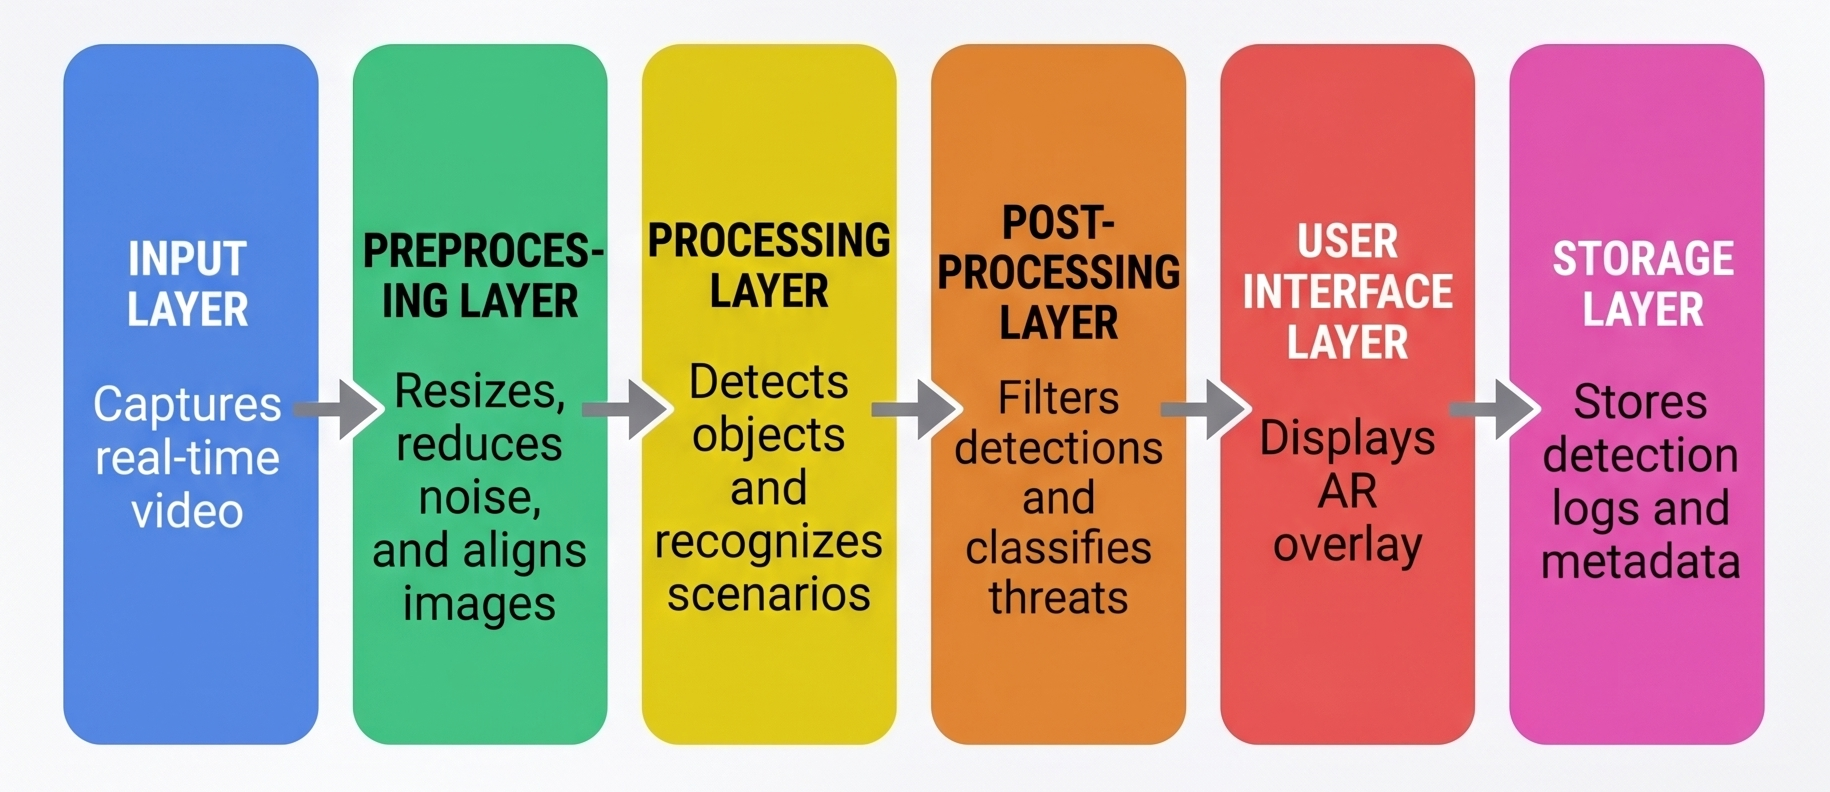
\includegraphics[width=0.9\textwidth]{images/architecture.png}
  \caption{System Architecture}\label{fig:architecture}
\end{figure}

The system architecture for the project is structured into six distinct layers that facilitate a
smooth data flow from capture to storage. It begins with the Input Layer, which is responsible for
capturing real-time video footage. This raw data is then passed to the Preprocessing Layer, where
images are resized, aligned, and noise is reduced to ensure clarity for analysis. The Processing
Layer serves as the core intelligence hub, detecting objects and recognizing specific scenarios,
followed by the Post-Processing Layer, which filters these detections and classifies potential
threats. Finally, the User Interface Layer provides an interactive experience by displaying an AR
overlay of the results, while the Storage Layer logs all detection data and metadata for future
reference.

\label{end:architecture}
\section{System Workflow}\label{sec:workflow}
\begin{figure}[h]
  \centering
  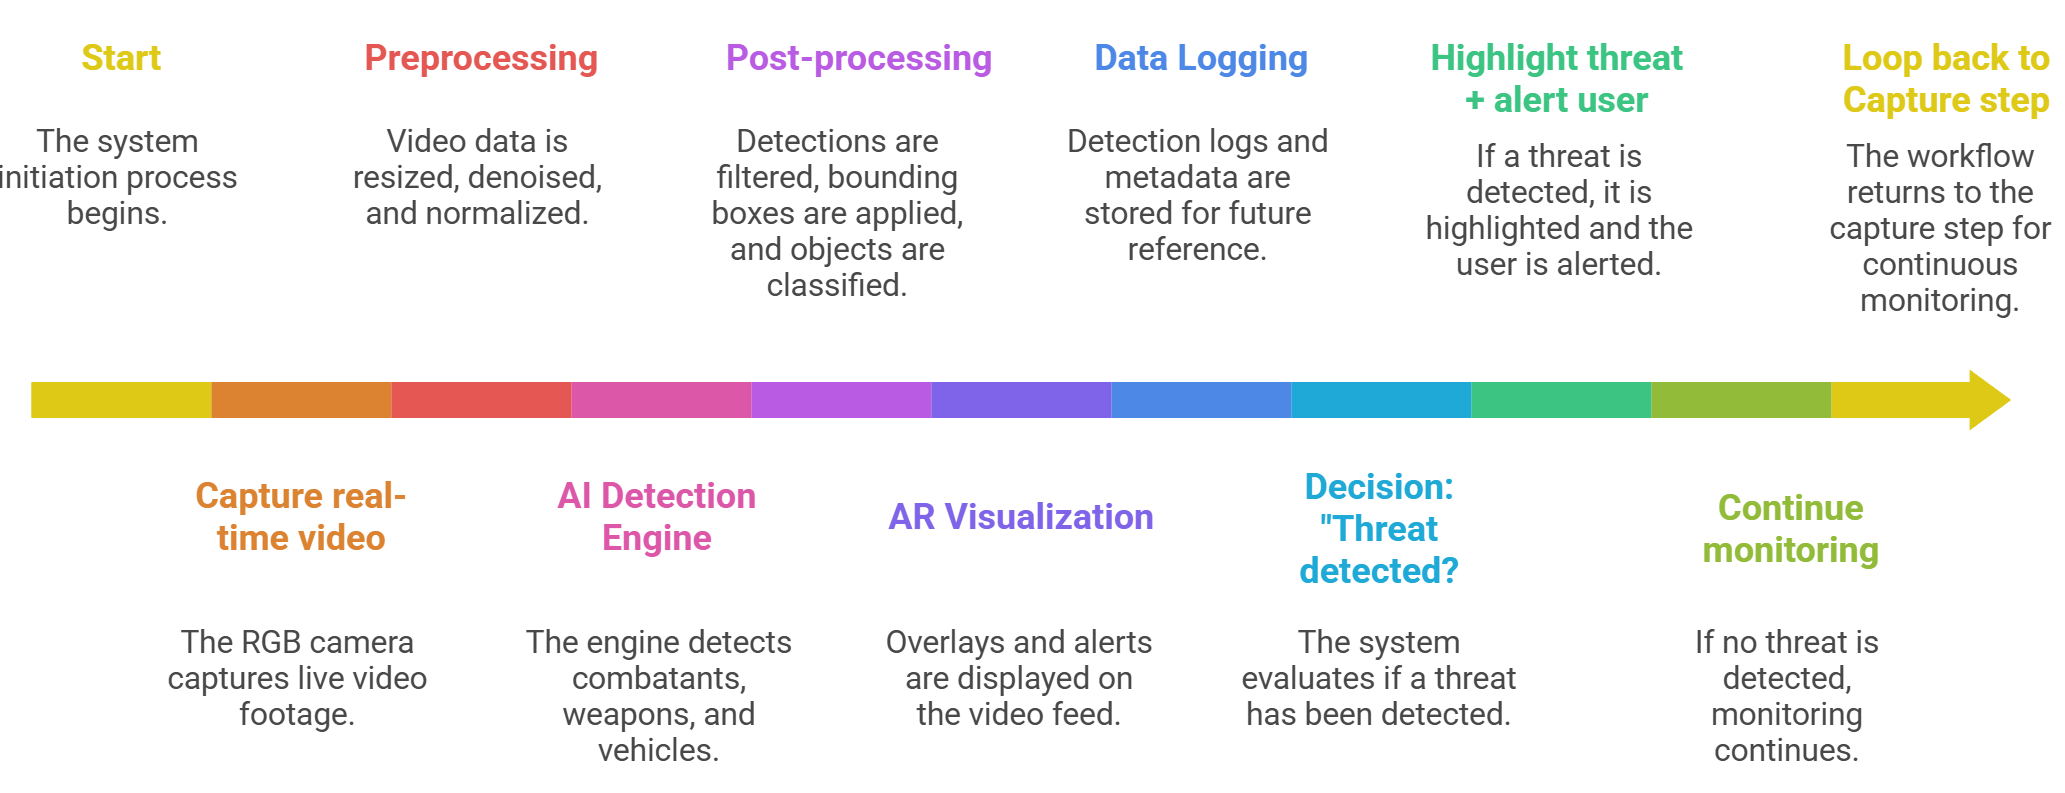
\includegraphics[width=0.9\textwidth]{images/workflow.png}
  \caption{System Workflow}\label{fig:workflow}
\end{figure}

The workflow follows a continuous loop designed for real-time monitoring and rapid response. Upon
initiation, the system captures live RGB video and immediately subjects it to preprocessing steps
like denoising and normalization. The AI Detection Engine then analyzes the feed to identify
combatants, weapons, or vehicles. This leads to a critical decision point: if a threat is detected,
the system applies bounding boxes, highlights the danger via AR visualization, alerts the user, and
logs the data. If no threat is found, the system simply continues its monitoring cycle, returning to
the capture step to ensure persistent surveillance.
\label{end:workflow}\label{end:design}

  \chapter{SCHEDULING}\label{ch:scheduling}

\section{Gantt Chart}\label{sec:gantt}
\begin{figure}[h]
  \centering
  \begin{ganttchart}[
    hgrid,
    vgrid,
    x unit=0.57\linewidth/16,
    title height=1
  ]{1}{20}

    \gantttitle{January}{4}
    \gantttitle{February}{4}
    \gantttitle{March}{4}
    \gantttitle{April}{4}
    \gantttitle{May}{4} \\

    \foreach \x in {1,...,5} {
      \gantttitlelist{1,...,4}{1}
    } \\

    \ganttbar[bar/.style={fill=violet!66, draw=black}]{Literature Survey}{3}{5} \\
    \ganttbar[bar/.style={fill=blue!66, draw=black}]{Base Paper Selection}{5}{6} \\
    \ganttbar[bar/.style={fill=green!66, draw=black}]{Supp. Papers Selection}{7}{13} \\
    \ganttbar[bar/.style={fill=yellow!66, draw=black}]{Report Drafting}{12}{15} \\
    \ganttbar[bar/.style={fill=orange!66, draw=black}]{Report Finalization}{16}{16} \\
    \ganttbar[bar/.style={fill=red!66, draw=black}]{Report Submission}{17}{18}
  \end{ganttchart}

  \caption{Gantt Chart for Major Project (Phase-1)}\label{fig:gantt}
\end{figure}

The project follows a structured timeline spanning from January to May. The initial phase begins in
the second week of January with a three-week Literature Survey, which concludes in early February.
This is immediately followed by the Base Paper Selection, spanning the first two weeks of February.
Supporting Papers Selection constitutes the longest research block, starting in late February and
continuing through the end of April. As research nears completion, Report Drafting commences in
early April and runs for three weeks. The final stages are tightly scheduled in May, with Report
Finalization occurring in the first week, followed by the final Report Submission during the second
and third weeks of the month. This sequential approach ensures a rigorous foundation of research
before the final documentation is prepared and delivered.

\label{end:gantt}
\section{Month-wise Progress}\label{sec:progress}
The project timeline spans from January to May 2026, transitioning from initial literature research
to final documentation. The month-wise progress details are as follows:

\subsection{January}
Conducted a comprehensive literature survey to identify relevant research papers and technologies in
the domain of real-time combat vision systems. Identified research papers that could serve as the
base paper and foundation for our project.

\subsection{February}
Selected the base paper and conducted extensive reading and analysis to understand the current state
of the art, identify gaps in existing solutions, and select a base paper that aligns with our
project objectives.

\subsection{March}
Selected 10 supplementary papers that provide additional insights, methodologies, and technologies
relevant to our project. These papers contribute to the development of our combat vision system by
providing a broader understanding of the field and potential approaches to implementation. Began
intial work to draft the project report.

\subsection{April}
Drafted the project report, synthesizing information from the base paper and supplementary papers.
Structured the report to clearly articulate the project details and specifications. Iteratively
refined the report based on feedback and additional insights gained during the drafting process and
drafted the final project report.

\subsection{May}
\begingroup\emergencystretch=2em
  Submitted the finalized project report, ensuring that all sections are complete, well-organized,
  and adhere to the required guidelines.
  \label{end:progress}\label{end:scheduling}
\par\endgroup

  \chapter{CONCLUSION}\label{ch:conclusion}
The project advances tactical situational awareness by combining state-of-the-art AI with wearable
combat technology. It employs the lightweight YOLOv8 architecture and multimodal image fusion to
enable real-time, autonomous threat detection in high-stress environments. By integrating visible
and thermal imaging, the system remains effective in challenging conditions such as darkness, smoke,
and low visibility. This reduces cognitive load on personnel by converting complex visual data into
actionable insights, enabling faster and more accurate decision-making. The system’s robustness is
enhanced through GAN-based synthetic data augmentation, which addresses limited military datasets,
and CLIP-based open-vocabulary detection, allowing adaptation to unseen threats via natural language
guidance. Additionally, its edge-optimized design enables high-speed, low-latency inference on
portable, smartphone-based hardware. This ensures reliable performance even in signal-denied
environments while maintaining data security and operational efficiency, ultimately supporting rapid
and informed responses in critical combat scenarios. \vspace{6pt}

Looking forward, the potential for VeerDrishti extends into a scalable framework for future defense
innovations. Future iterations could integrate more complex action recognition models to predict
hostile intent or incorporate advanced feature-fusion strategies to further enhance the detection of
micro-scale targets. In conclusion, VeerDrishti offers a versatile and reliable solution for modern
national security. By harmonizing cutting-edge computer vision research with the practical,
high-stakes requirements of the frontline, the project provides a definitive technological
advantage, ensuring enhanced safety and operational efficiency for ground units in the evolving
landscape of modern warfare.
\label{end:conclusion}

  \defbibheading{bibintoc}[REFERENCES]{%
    \chapter*{#1}\addcontentsline{toc}{chapter}{#1}\label{ch:references}}
  \begingroup
    \emergencystretch=2em
    \printbibliography[heading=bibintoc,title={REFERENCES}]
    \label{end:references}
  \endgroup
\end{document}
